\subsubsection*{4a) Synchronization}

Ensure data consistency \& correct execution order when multiple threads / processes access shared data concurrently. Handles ordering, timing, mutual exclusion.

\textbf{Cooperating processes} execute concurrently; \textbf{shared data} access can lead to \textbf{race conditions} (unpredictable behavior). A \textbf{data race} occurs when two+ threads access the same memory, one writes, without proper ordering. \textbf{Critical section (CS)}: only one process at a time; must ensure \textbf{mutual exclusion}, \textbf{progress}, and \textbf{bounded waiting}.  

\textbf{Peterson's solution}: for 2 processes, uses \textbf{flags} and \textbf{turn} for atomic control.

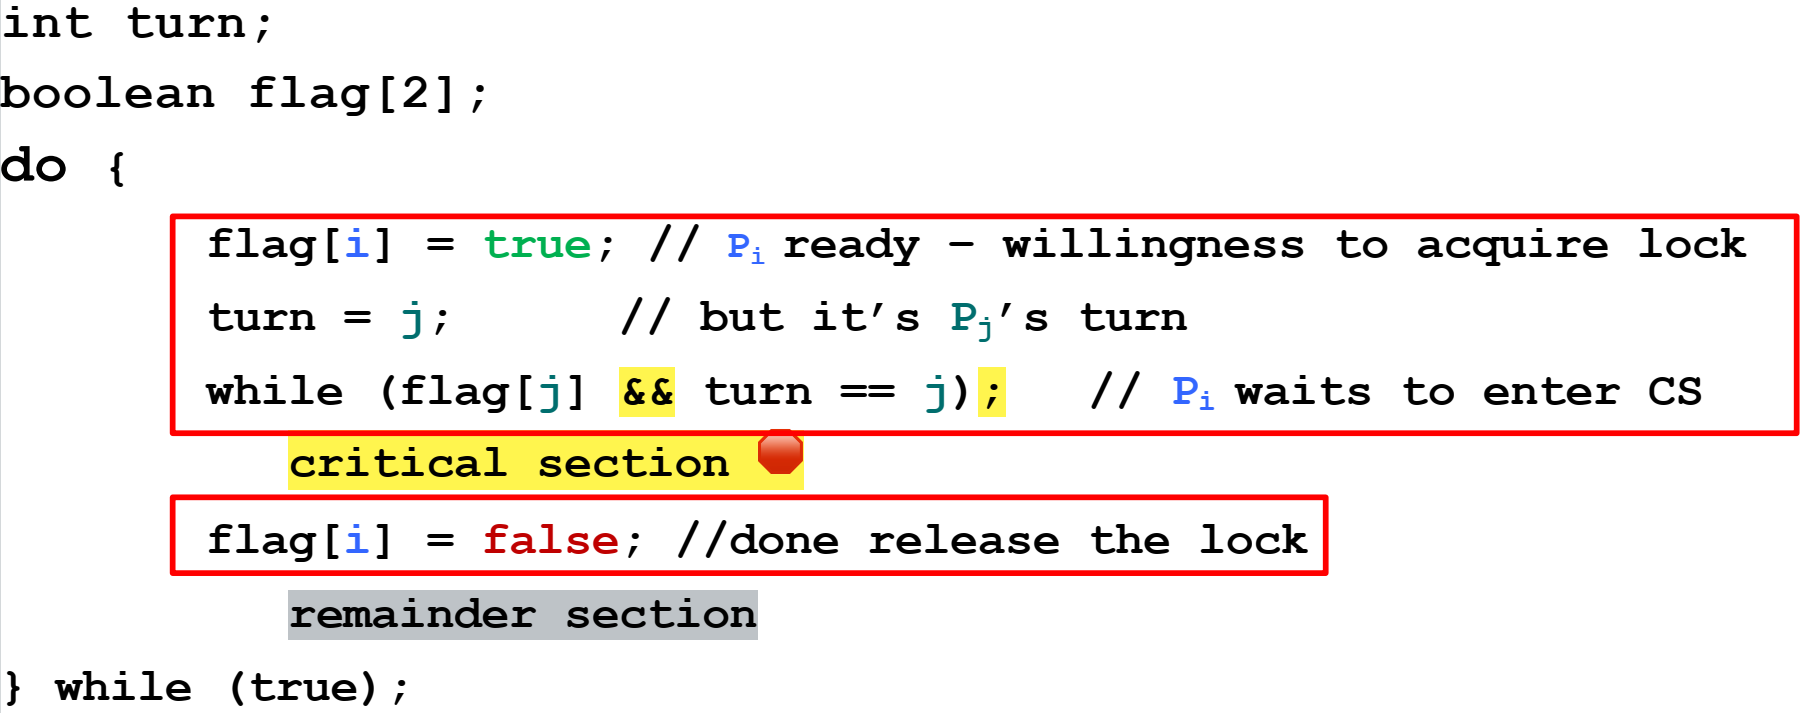
\includegraphics[width=0.95\linewidth]{images/04a_p17_peterson.png}

\textbf{Mutex}: acquire/release lock for CS; \textbf{spinlocks} use busy waiting, preferred for short waits on SMP (Symmetric Multiprocessing).

\textbf{Semaphores}: integer S, \textbf{wait} decrements, \textbf{signal} increments; can block processes in a waiting queue. Avoids busy waiting at app level but risks \textbf{deadlocks} and \textbf{starvation}.

\textbf{Priority inversion}: low-prio holds lock needed by high-prio. 
\textbf{Bounded}: high-prio blocked by low-prio.
\textbf{Unbounded}: mid-prio preempts low-prio, extending high-prio wait. Solved by \textbf{PIP} (priority inheritance protocol) or \textbf{PCP} (priority ceiling protocol).

\textbf{Monitors}: high-level abstraction ensuring mutual exclusion; includes \textbf{condition variables} (x.wait, x.signal) for coordination.
Only one process active in monitor at a time.
Unlike semaphores, signal() has no effect if no process is waiting. 

Problems: 1) Access without permission, 2) Never release resource, 3) Release not-held resource, 4) Request same resource multiple times.


\subsubsection*{4b) Examples}
\textbf{Bounded buffer}: producer-consumer problem, \textbf{binary/counting semaphores} or \textbf{mutex locks} solve access control.

mutex = 1;
empty = n;
full = 0;

Producer:
wait(empty);
wait(mutex);
\textit{// add item}
signal(mutex);
signal(full);

Consumer:
wait(full);
wait(mutex);
\textit{// remove item}
signal(mutex);
signal(empty);

\textbf{Philosophers}: prevent \textbf{deadlock} and \textbf{starvation}; 5 philosophers, 5 chopsticks. All grabbing left chopstick: deadlock. Avoid: allow max 4 to eat, \textbf{asymmetric solution} (odd eat directly), \textbf{condition self[i]} for permission, ensure \textbf{mutual exclusion}, but can violate \textbf{bounded waiting}.

\textbf{Linux}: pre-2.6 \textbf{nonpreemptive kernel} with small CS. Provides \textbf{atomic\_t}, \textbf{spinlocks}, \textbf{semaphores}, \textbf{mutexes}. Spinlocks avoid complex locks, deterministic; needed on \textbf{SMP} for race conditions. Spinlock: acquire = disable preemption, release = enable.

\textbf{POSIX}: \textbf{named semaphores} via \texttt{sem\_open()}, unnamed via shared memory \texttt{sem\_init()}.

\textbf{OpenMP}: \textbf{compiler directives} and API; \texttt{\#pragma omp critical} or \texttt{omp atomic} for lightweight, non-blocking synch.


\subsubsection*{4c) Deadlocks}
\textbf{Deadlock}: multiple \textbf{resources} (CPU, IO, mem), multiple instances. Process \textbf{requests} (open, allocate, wait), \textbf{uses}, then \textbf{releases} (close, free, signal). 
Example: thread1 locks A then B; thread2 locks B then A → circular wait.

\textbf{Livelock}: process proceeds but no progress, often due to lock contention.
Analogy: Two people in a hallway stepping side to side, never passing.
Solution: Add randomness/asymmetry (like dining philosophers) to break the cycle.
Deadlock = waiting indefinitely. Livelock = doing actions repeatedly but no progress.

In multithreading: mutex via \texttt{pthread\_mutex\_t}, use \texttt{\_init}, \texttt{\_lock}, \texttt{\_unlock}. DL occurs when one locks first and second locks second, circular blocking.

\textbf{DL conditions}
(Only if all four conditions are present, deadlock may occur)\\
- \textbf{Mutual exclusion}: Some resources can only be held by one process at a time.\\
- \textbf{Hold \& Wait}: A process holding at least one resource is waiting for additional resources held by other processes.\\
- \textbf{No preemption}: Resources can't be forcibly taken; they must be released voluntarily.\\
- \textbf{Circular wait}: A circular chain of processes exists, each waiting for a resource held by the next one in the chain.\\

DL handling:\\
1. Prevention/Avoidance (protocols)\\
2. Detection \& Recovery\\
3. Ignore (programmer responsible) 

Prevention: break 1 of 4 conditions. \textbf{1. Mutual exclusion} (can't), \textbf{2. Hold \& wait} (request all at once), \textbf{3. Preemption} (release all on failure, often impractical), \textbf{4. Resource ordering} (unique int IDs, acquire in order).
